\chapter{INTRODUCTION}
\label{sec:introduction}
\section{Scientific/Technical Background}

Gases in the stratosphere play a pivotal role in climate modelling due to their prolonged lifetime.
Especially methane sources have been shown to play a big role in climate modelling \cite{stocker2013, saunois2017, nisbet2019, turner2019}. Since remote sensing via satellites is used to monitor methane sources and sinks on a large scale they contribute a lot to climate models. However, they heavily depend on atmospheric models to compute the methane concentrations at different altitudes from the averaged column densities they can measure. Therefore, more accurate in-situ measurements of methane are needed, which was reflected on in the National Research Council Decadal Survey for Earth Science \cite{national2019} and the summary report by the Carbon Climate Workshop in 2018 \cite{sellers2018}. 

The concentration of atmospheric methane ranges from around 2 ppm down to 0.7 ppm between 0 and 30 km altitude.
Because of the small concentrations, accurate optically complex systems like \gls{tdlas} \cite{joly2020} or \gls{ftir} \cite{runge2023} are widely employed.
\gls{tdlas} systems send a laser beam of varying frequency close to the excitation energy of the target molecule through a gas sample and calculate the target molecule's concentration based on the measured absorption via the Beer-Lambert law.
\gls{ftir} works by sending a light beam containing multiple frequencies into the gas sample and recording the total absorption.
The frequencies are then changed and the process repeated.
This is often done via a Michelson interferometer.
Both techniques have the potential to enable great accuracy depending on their path length. However, to get longer pathlengths it is often necessary to reflect the laser beam thousands of times since measurements are usually limited in space. Therefore, high precision is required in the complex optical setups, meaning that those systems are expensive, inaccessible and often highly sensitive to vibrations and shocks.

During recent years, \gls{ndir} sensors have advanced as a cost-effective and simple alternative to laser-based devices commonly employed for methane sensing.
NDIR spectroscopy works by passing a spectrum of \gls{ir} light through a gas sample where each gas absorbs the light at a unique wavelength.
An optical filter selects the wavelengths of the gas of interest.
The intensity of the transmitted light at the relevant wavelength can then be measured to receive the absorbance $A=\log_{10}\left(\frac{I_0}{I}\right) = c\varepsilon l$.
The concentration c of the gas can then be calculated using the Beer-Lambert law

\begin{equation}
c = \log_{10}\left( \frac{I_{0}}{I} \right) \times {(\varepsilon l)}^{- 1},
\end{equation}

where $\varepsilon$ is the molar absorption coefficient, specific to the gas species, $l$ is the path length between light source and detector and $I_{0}$ and $I$ are the initial intensity of light and the intensity at the detector.
$I_{0}$ is determined either before the measurement or simultaneously using a second detector.
A schematic is provided in Figure \ref{fig:ndir_principle}.
Due to the simple setup, the overall cost of NDIR detectors is quite small with a range of tens to a few 100s of Euros. Furthermore, using a simple setup with a broad light sources, makes the device more robust against misalignment.

\begin{figure}[htbp]
\centering
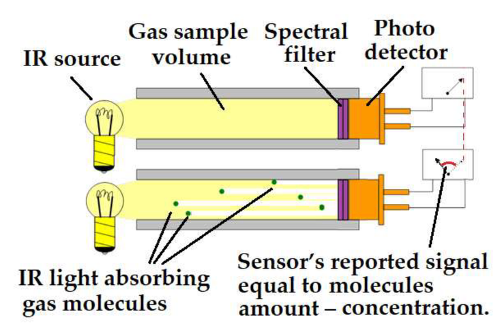
\includegraphics[width=8cm]{0_images/figures/NDIR schematic.png}
\caption{Schematic of the non-dispersive infrared (NDIR) measurement principle.
Source: \cite{gaynullin2025}}
\label{fig:ndir_principle}
\end{figure}

At the same time, less reflections mean a shorter pathlength and a broader wavelength spectrum means limited applicability of the Beer-Lambert law. Another drawback of having a light source with a broader spectrum (compared to a laser) is that the absorption spectra of several molecules can overlap and make it harder to differentiate the effect of different absorbing molecules. In the case of methane, there is a large overlap with water molecules, which are usually present in a far bigger concentration in the atmosphere. This has previously limited NDIR so much that it couldn't be applied to measuring atmospheric methane. \\
\begin{figure}[htbp]
\centering
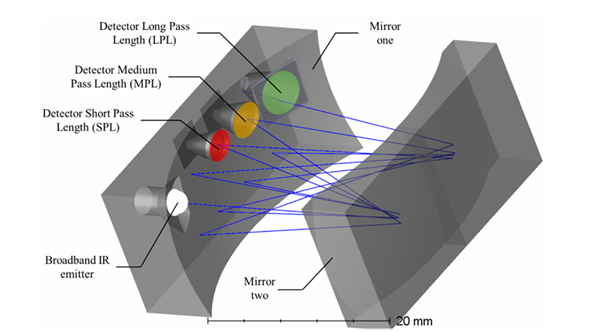
\includegraphics[width=8cm]{0_images/figures/K96principle.png}
\caption{Schematic of K96 sensor core, which combines three detectors for water, carbon dioxide and methane.
Source: \cite{wastine2022}}
\label{fig:K96_principle}
\end{figure}

However, recently a new sensor has been developed by Senseair AB \cite{wastine2022}, which measures $\mathrm{CH_4}$, $\mathrm{H_2 O}$, and $\mathrm{CO_2}$ at the same time by using three different detectors in one sensor core as depicted in \autoref{fig:K96_principle}. This allows one to subtract the influence of water and carbon dioxide absorption from the methane signal. Therefore, this NDIR sensor is a promising candidate for atmospheric methane monitoring. \\  
While the K96 sensor is a state of the art sensor and delivers higher resolution methane measurements than other NDIR sensors, it is not quite accurate enough to measure atmospheric methane concentrations reliably. The \gls{lod}, which gives the lowest concentration at atmospheric pressures that can be detected by the K96 sensor is about 3\,ppm\cite{mao_improvement_2025}. Therefore, it is necessary to increase the concentration. Here it is important to differentiate the terms concentration and molar fraction, which are often used interchangeably because most contexts are working under ground level conditions with a constant pressure. While concentration gives the particle number per volume $c=\frac{n}{V}$, the molar fraction means particle number of a certain gas species per total particle number including all present gas species $x_i=\frac{n_i}{n_{tot}}$. When a detector resolution is given in particles-per-million or ppm, this is usually assumed for ground level. In reality the quantity of interest for an optical sensor that is based on the Beer-Lambert law is the concentration of the gas species.\\ 
Now, since the pressure $p$ decreases exponentially with altitude, the concentration

\begin{equation}
c = \frac{n}{V}
\end{equation}

connected to the pressure by the ideal gas law

\begin{equation}
pV = nRT
\end{equation}

with the volume $V$, the ideal gas constant $R$ and the temperature $T$, decreases with about the same rate as the pressure. If it were assumed that the composition of the air stayed constant, the molar fraction would not be affected by this drop in the particle number. However, the emitted light would now encounter way fewer particles and therefore be less absorbed. This means that a detector with low accuracy has an even lower signal if the pressure drops. Furthermore, the relative molar fraction of methane molecules compared to other molecules in the air is actually decreasing from 2\,ppm to about 1\,ppm as the atmospheric composition changes between Troposphere and Stratosphere, which means that there are even fewer methane molecules at the altitudes reached by the BEXUS gondola.\\
Therefore it is necessary to pressurise the air to increase the concentration of methane particles. Due to the \gls{lod} of the K96 of 3\,ppm it is not enough to keep the pressure at 1\,bar. Instead it is necessary to increase the pressure to at least 3\,bar to be able to measure with the K96 even at altitudes of 20\,km where the molar fraction could be already as low as 1\,ppm. Having a pressure of 3 bar in the measurement chamber would increase the "effective molar fraction" to 3\,ppm in that case, just high enough to rely on the sensor. \\
The sensor is susceptible to other factors causing drift such as temperature and humidity. These will require a thorough calibration strategy, which allows to measure the methane concentration under varying conditions. An AI-based calibration approach has been tested before on the K96 sensor\cite{gia_accurate_2025} and therefore a similar approach could be employed for \gls{mirage}. At the same time, the experiment should limit the temperature range of the air to be measured, which requires a thermal control system.\\



%%%%%%%%%%%%%%%%%%%%%%%%%%%%%%%%%%%%%%%%%%%%%%%%%%%%%%%%%%%%%%%%%%%%%%%%%%%%%%%
\section{Mission Statement}

As explained in Section 1.1 methane measurements are of great importance for climate modelling.
However, systems with which methane measurements are taken, are oftentimes expensive and complex in setup.
Therefore, \gls{mirage} aims to demonstrate a low-cost, low-complexity solution for measuring methane concentrations in the upper stratosphere.
By using the novel K96 non-dispersive infrared (NDIR) sensor developed by Senseair AB (a Swedish company, specialised in state-of-the-art gas sensors) \cite{wastine2022} off-the-shelf technology will be shown to provide an alternative to laser-based approaches.

%%%%%%%%%%%%%%%%%%%%%%%%%%%%%%%%%%%%%%%%%%%%%%%%%%%%%%%%%%%%%%%%%%%%%%%%%%%%%%%
\section{Experiment Objectives}

\begin{table}[H]
\centering
\caption{Experimental Objectives}
\label{tab:objectives}
\begin{tabularx}{0.9\textwidth}{lX}
\toprule
\textbf{Priority} & \textbf{Description} \\
\midrule
Technical - Primary & Measure methane, carbon dioxide and water with an NDIR sensor core up to at least 20\,km altitude.\\
Technical - Primary & Demonstrate a pressurisation system that can maintain 3 bar up to at least 20km altitude.\\
Scientific - Secondary & Validate recorded measurements via chemical transport models, satellite data and previous in-situ measurements by other groups.\\
Scientific - Secondary & Evaluate decrease of measurement uncertainty in the field by employing AI-based calibration.\\
\bottomrule
\end{tabularx}
\end{table}

%%%%%%%%%%%%%%%%%%%%%%%%%%%%%%%%%%%%%%%%%%%%%%%%%%%%%%%%%%%%%%%%%%%%%%%%%%%%%%%
\section{Experiment Concept}

The Non-Dispersive Infra-Red (NDIR) sensor detects light absorption due to the number of absorbing particles in the optical cavity within a narrow wavelength range.
As mentioned in Section 1.1, this number is related to the concentration of the contributing gas species and their pressures and temperature.
Thus, it is possible to increase the concentration of a gas species by increasing the pressure of the gas while maintaining the same relative composition and molar fractions of the sample.

Therefore, an NDIR sensor fed with pressurized ambient air under temperature-controlled conditions will be used. To keep a pressure of 3\,bar up to at least 20\,km altitude is the real challenge of \gls{mirage}. As explained above, ambient air needs to be pressurized to 3 bar using a combination of vacuum pumps and a compressor, that work together. Vacuum pumps are meant to draw in low density ambient air and pre-pressurise this air to provide air dense enough for the compressor to further pressurise it to 3 bar. Air can leave the pressurized chamber through a valve, which could be passive since the outflow rate is independent of altitude since it is limited by the speed of sound even if the pressure difference is just 2 bar as it will be on ground level. The concept and different components involved in the pressurisation system will be explained in more depth in the mechanical design section below. \\
To stabilize the temperature of the air is another complex challenge, that needs to be solved via a thermal control system, that can handle varying ambient conditions. The air is initially very cold with a low density but due to pressurisation it can heat up substantially. At the same time, it's mass is small and it will lose heat to surrounding tubing and chamber walls. Electrical components such as pumps, that are also generating heat and active and passive heating elements need to make sure that the air is cooled and heated to the right temperatures in the right places. An extensive thermal study including more factors will analyse the thermal system needed further in the thermal design section below.\\
Additionally, information is needed about the ambient pressure and temperature, to inform the thermal control system and the flow rate of the pumps. Furthermore, this allows for calculation of the concentration of the methane particles outside of the experiment from the concentration measured via the ideal gas law.\\
As water vapor is a major factor in the uncertainty of the sensor and condensation of water could damage the sensor and other electronics, the inside and ideally outside humidity should be monitored as well.
These measurements can then be used to engage mitigation methods like closing the vent, stopping the pumps and raising the internal temperature to increase the water capacity of the air and prevent further condensation. Once the ambient humidity sensor is reporting safe levels, the pressurisation system can start working again, flushing out the more humid air. The internal temperature is to be set to normal operating conditions again as well. \\
Many sensors will be required to monitor those different ambient conditions and internal temperature, pressure and humidity. Depending on the location within the setup they need to be able to work under different conditions and fulfill different accuracy and range requirements. An analysis of their selection and the state of the art is done in the electrical design section below.\\
A \gls{mcu} will be integrated into a PCB designed to handle all of the different processes that the experiment has to fulfill to ensure reliable measurements of the atmospheric methane concentrations up to an altitude of at least 20\,km.  
A block diagram showcasing the different functional/physical experiment blocks is provided below in Figure \ref{fig:block_diagram}.

\begin{figure}[t]
\centering
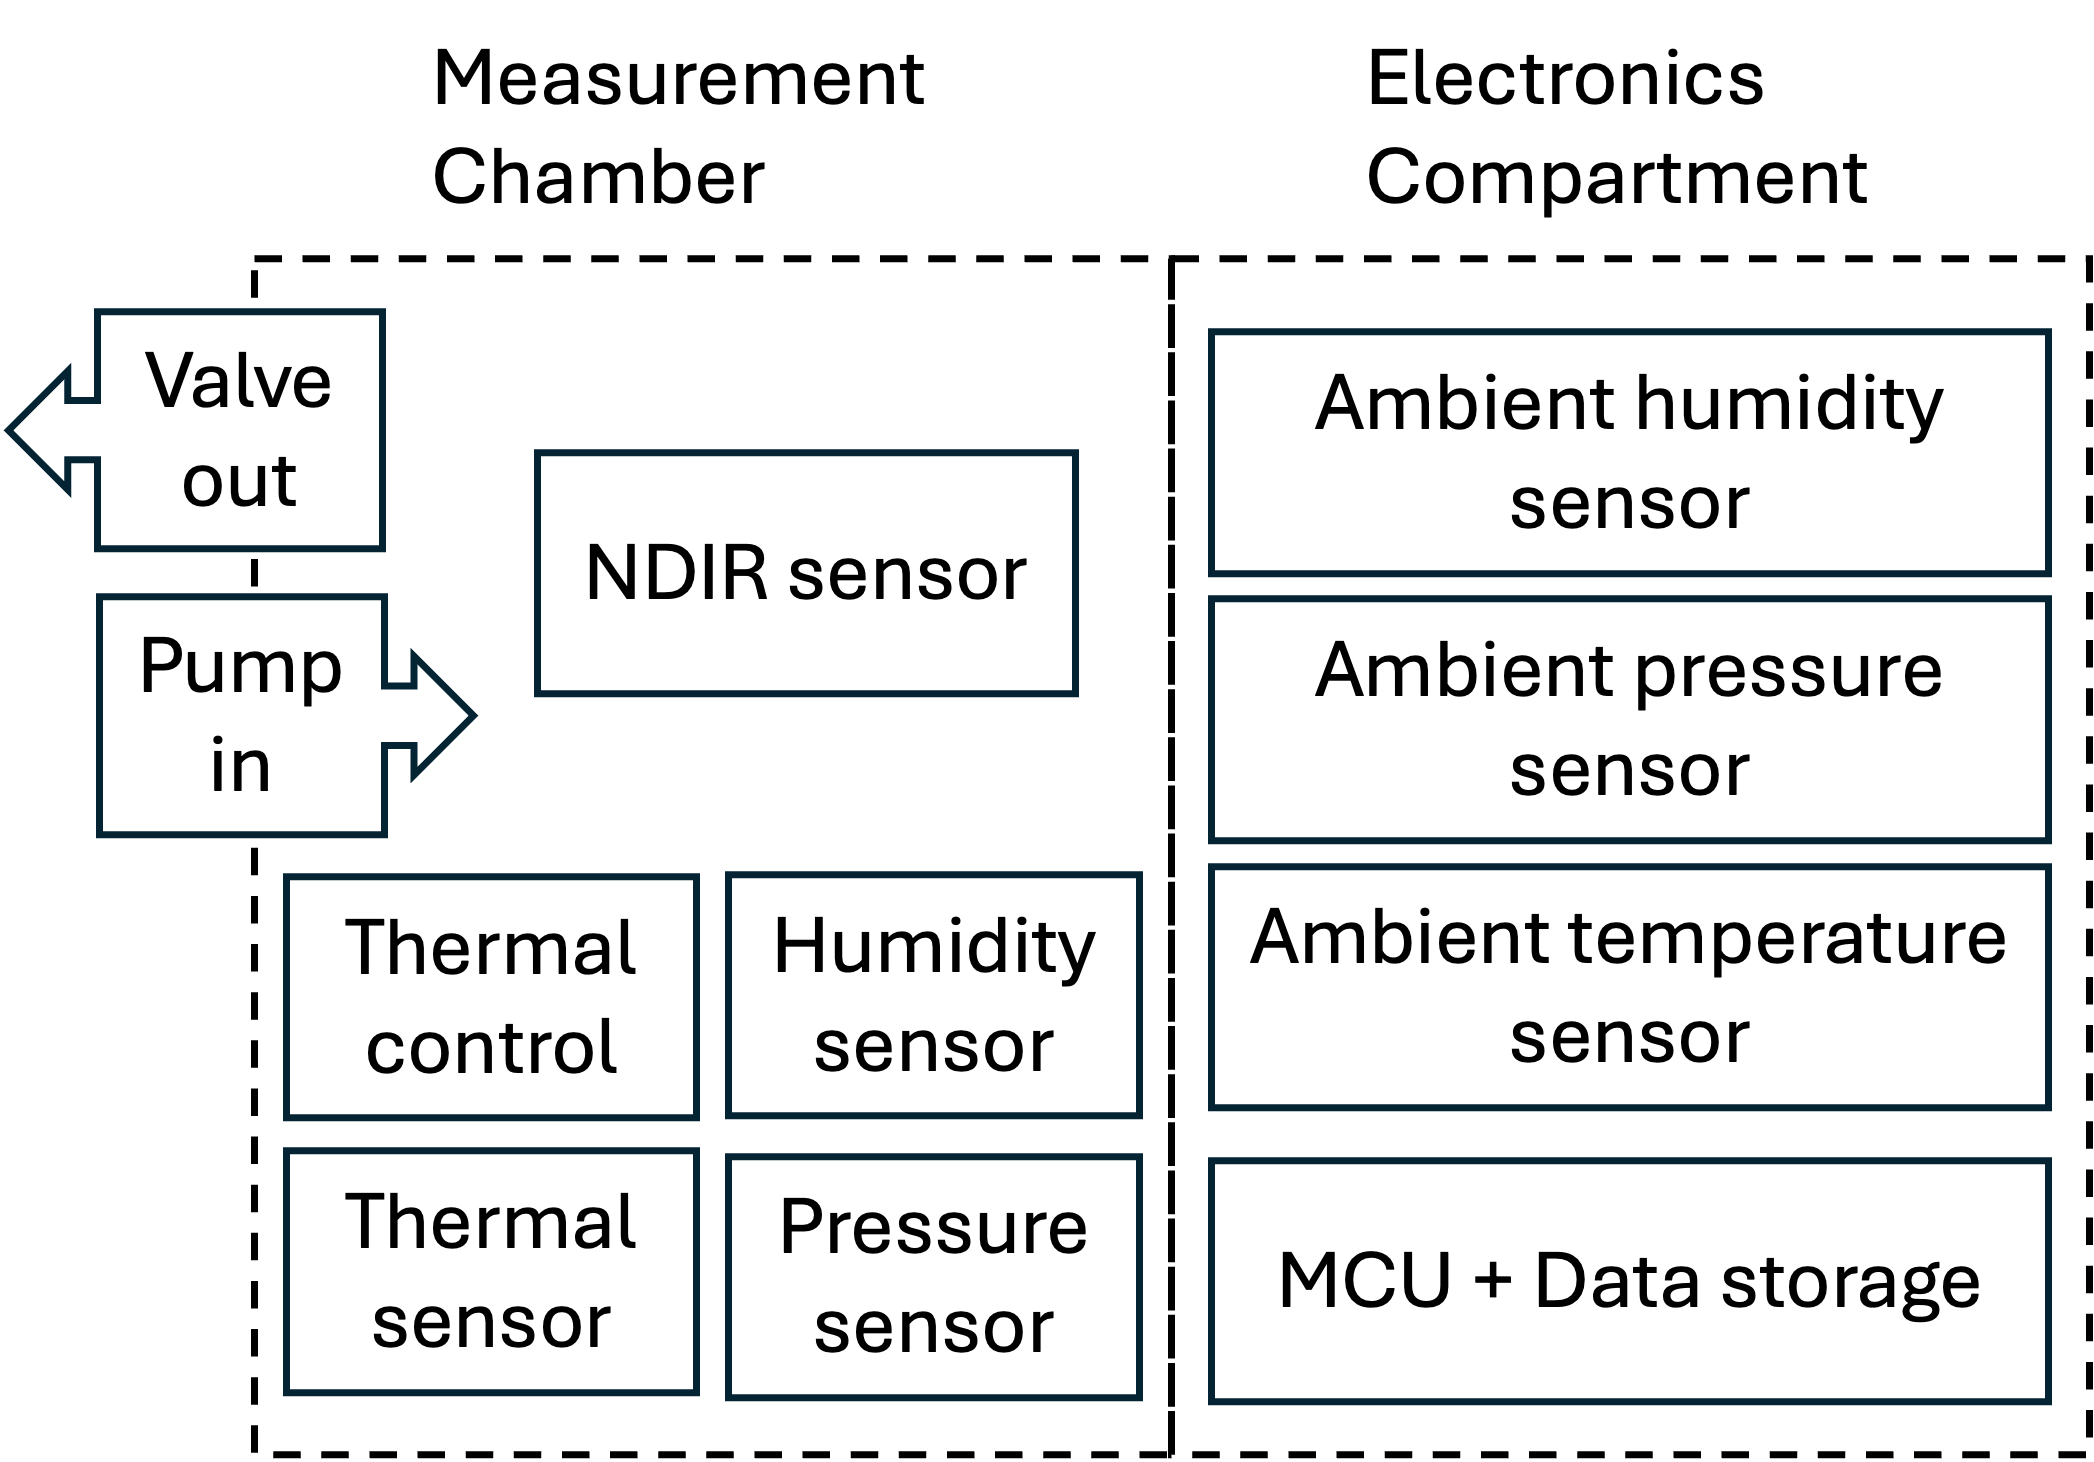
\includegraphics[width=\textwidth]{0_images/figures/Components block diagram.png}
\caption{Block diagram with different physical or functional components of the experiment.}
\label{fig:block_diagram}
\end{figure}

%%%%%%%%%%%%%%%%%%%%%%%%%%%%%%%%%%%%%%%%%%%%%%%%%%%%%%%%%%%%%%%%%%%%%%%%%%%%%%%
\section{Team Details}

The team of \gls{mirage} is still in the process of recruiting team members, especially for the bachelor thesis projects.
All team members are studying at Uppsala University.

%%%%%%%%%%%%%%%%%%%%%%%%%%%%%%%%%%%%%%%%%%%%%%%%%%%%%%%%%%%%%%%%%%%%%%%%%%%%%%%
\subsection{Contact point}

Team leader phone number: +46 76 456 08 02\\
Email: abdullah.alsakka.5356@student.uu.se\\
Team leader address: Studentvägen 18, Uppsala SE75234

%%%%%%%%%%%%%%%%%%%%%%%%%%%%%%%%%%%%%%%%%%%%%%%%%%%%%%%%%%%%%%%%%%%%%%%%%%%%%%%
\subsection{Team Members}

\begin{itemize}
    \item \textbf{Name:} Abdullah Alsakka \\
    \textbf{Education (Year):} Masters in Astronomy and Space Physics (2\textsuperscript{nd} year) \\
    \textbf{Role:} Team Leader and Science team

    \item \textbf{Name:} Jonathan Remmert \\
    \textbf{Education (Year):} Masters in Astronomy and Space Physics (2\textsuperscript{nd} year) \\
    \textbf{Role:} Science team
    
    \item \textbf{Name:} Oliver Bolin \\
    \textbf{Education (Year):} Electrical Engineering (2\textsuperscript{nd} year/ 5 year program) \\
    \textbf{Role:} Electrical Team
    
    \item \textbf{Name:} Max Steen \\
    \textbf{Education (Year):} Electrical Engineering (2\textsuperscript{nd} year/ 5 year program) \\
    \textbf{Role:} Electrical Team

    \item \textbf{Name:} Anna Tschesche \\
    \textbf{Education (Year):} Master in Material Science (2\textsuperscript{nd} year) \\
    \textbf{Role:} Science Team

    \item \textbf{Name:} Olle Hallberg \\
    \textbf{Education (Year):} Engineering Physics (3\textsuperscript{rd} year/ 5 year program) \\
    \textbf{Role:} Science Team

    \item \textbf{Name:} Molly Sundell \\
    \textbf{Education (Year):} Material Engineering (3\textsuperscript{rd} year/ 5 year program) \\
    \textbf{Role:} Outreach Team

    \item \textbf{Name:} Antoni Marciniewski \\
    \textbf{Education (Year):} Mechanical Engineering (1\textsuperscript{st} year) \\
    \textbf{Role:} Mechanical Team

    \item \textbf{Name:} Leo Adolphus Wattin \\
    \textbf{Education (Year):} Mechanical Engineering (2\textsuperscript{nd} year) \\
    \textbf{Role:} Mechanical Team

    \item \textbf{Name:} Lydia Lindeberg-Lindvet \\
    \textbf{Education (Year):} Engineering Physics (3\textsuperscript{rd} year/ 5 year program) \\
    \textbf{Role:} Software Team

    \item \textbf{Name:} Karl Johansson \\
    \textbf{Education (Year):} Engineering Physics (3\textsuperscript{rd} year/ 5 year program) \\
    \textbf{Role:} Software Team

    \item \textbf{Name:} Joel Harknäs \\
    \textbf{Education (Year):} Engineering Physics (3\textsuperscript{rd} year/ 5 year program) \\
    \textbf{Role:} Electrical Team

    \item \textbf{Name:} Egon Bertilsson \\
    \textbf{Education (Year):} Engineering Physics (3\textsuperscript{rd} year/ 5 year program) \\
    \textbf{Role:} Electrical Team

    \item \textbf{Name:} Hugo Hansson \\
    \textbf{Education (Year):} Engineering Physics (3\textsuperscript{rd} year/ 5 year program) \\
    \textbf{Role:} Electrical Team

    \item \textbf{Name:} Sebastian Christensson \\
    \textbf{Education (Year):} Electrical Engineering (3\textsuperscript{rd} year/ 5 year program) \\
    \textbf{Role:} Electrical Team

    \item \textbf{Name:} Maximilian Fröderberg-Dramberg \\
    \textbf{Education (Year):} Electrical Engineering (3\textsuperscript{rd} year/ 5 year program) \\
    \textbf{Role:} Electrical Team

    \item \textbf{Name:} David Sivertsen \\
    \textbf{Education (Year):} Electrical Engineering (3\textsuperscript{rd} year/ 5 year program) \\
    \textbf{Role:} Electrical Team

    \item \textbf{Name:} Sixten Sundsten \\
    \textbf{Education (Year):} Electrical Engineering (3\textsuperscript{rd} year/ 5 year program) \\
    \textbf{Role:} Electrical Team

    \item \textbf{Name:} Axel Lindblom \\
    \textbf{Education (Year):} Electrical Engineering (3\textsuperscript{rd} year/ 5 year program) \\
    \textbf{Role:} Electrical Team

    \item \textbf{Name:} Haya Basunaid \\
    \textbf{Education (Year):} Material Engineering (3\textsuperscript{rd} year/ 5 year program) \\
    \textbf{Role:} Mechanical Team

    \item \textbf{Name:} Robin Jensen \\
    \textbf{Education (Year):} Mechanical Engineering (3\textsuperscript{rd} year) \\
    \textbf{Role:} Mechanical Team

    \item \textbf{Name:} Marcus Gathe \\
    \textbf{Education (Year):} Mechanical Engineering (3\textsuperscript{rd} year) \\
    \textbf{Role:} Mechanical Team

    \item \textbf{Name:} Pelle Lindvall \\
    \textbf{Education (Year):} Mechanical Engineering (3\textsuperscript{rd} year) \\
    \textbf{Role:} Mechanical Team

    \item \textbf{Name:} Björn Hagland \\
    \textbf{Education (Year):} Engineering Physics (3\textsuperscript{rd} year/ 5 year program) \\
    \textbf{Role:} Science Team
    
    \item \textbf{Name:} Albin Zetterquist \\
    \textbf{Education (Year):} Material Engineering (3\textsuperscript{rd} year/ 5 year program) \\
    \textbf{Role:} Science Team
\end{itemize}

%%%%%%%%%%%%%%%%%%%%%%%%%%%%%%%%%%%%%%%%%%%%%%%%%%%%%%%%%%%%%%%%%%%%%%%%%%%%%%%
\clearpage
